\chapter[Ferramentas de Gestão de Requisitos]{Ferramentas de Gestão de Requisitos}
\label{chap:ferramenta}
	Para um bom desenvolvimento do trabalho, foram avaliadas duas ferramentas para Gerência de Requisitos: VersionOne e Rally \emph{Software}.
	\\ \indent A ferramenta VersionOne foi indicada pelo grupo de monitores da equipe e a ferramenta Rally \emph{Software} foi descoberta em um artigo sobre discussão de metodologias ágeis. É importante ressaltar que as duas ferramentas lidam com contextos ágeis.
	\section[Análise de Ferramentas de Gestão de Requisitos]{Análise de Ferramentas de Gestão de Requisitos}
	\label{sec:ferramenta_analise}
		Nas subseções à seguir são descritas uma breve abordagem de cada ferramenta e os criterios adotados para avaliação.

		\subsection[A Ferramenta VersionOne]{A Ferramenta VersionOne}
		\label{subsec:ferramenta_analise_versionone}
			VersionOne é uma ferramenta de suporte ao desenvolvimento de \emph{software} utilizando metodologias ágeis, tais como Scrum, \emph{eXtreme Programming}, ou mesmo metodologias híbridas. De maneira geral, foi concebida para equipes pequenas de forma a promover a melhoria do processo de maneira fácil, rápida e inteligente.
			\\ \indent A ferramenta contém recursos de planejamento de \emph{releases}, \emph{sprints}, construção de \emph{roadmaps}, rastreamento de requisitos, etc. Uma ferramenta completa com recursos adequados para a utilização neste projeto. Contudo, a aprendizagem da utilização concisa da ferramenta poderia ficar comprometida, tendo em vista o tempo destinado à realização do trabalho.
			\\ \indent Segundo os idealizadores da ferramenta VersionOne, é possível perceber os seguintes pontos em relação à ferramenta:
			\begin{itemize}
				\item{Alavancar um único sistema para o planejamento e acompanhamento de todos os épicos, histórias, temas, defeitos, tarefas, testes e questões. O VersionOne fornece uma visibilidade entre várias equipes, projetos e portfólios ágeis, proporcionando um ambiente centralizado, onde todos os \emph{Stakeholders} - executivos, gerentes, proprietários do produto, desenvolvedores e testadores - podem facilmente trabalhar juntos, independentemente da localização;}
				\item{Construído a partir do zero para suportar os processos e fluxos de trabalho de desenvolvimento de \emph{software} ágeis, o VersionOne acelera a adoção da metodologia ágil. Há orientação para os membros da equipe em cada etapa do processo de desenvolvimento ágil. O VersionOne reforça continuamente as melhores práticas ágeis, sem ser prescritivo;}
				\item{Há possibilidade de fornecer às equipes a flexibilidade para trabalhar da maneira que elas querem. Fluxo de trabalho e espaços de trabalho personalizados. O VersionOne permite fazer o caminho ágil e adaptar os processos à medida que evoluem. Ao invés de impor a todos um tamanho único de abordagem, é possível selecionar a partir de modelos previamente concebidos e personalizados (metodologia Scrum, XP, Kanban, AgileUP, etc).}
			\end{itemize}
			\begin{figure}[h]
				\centering
				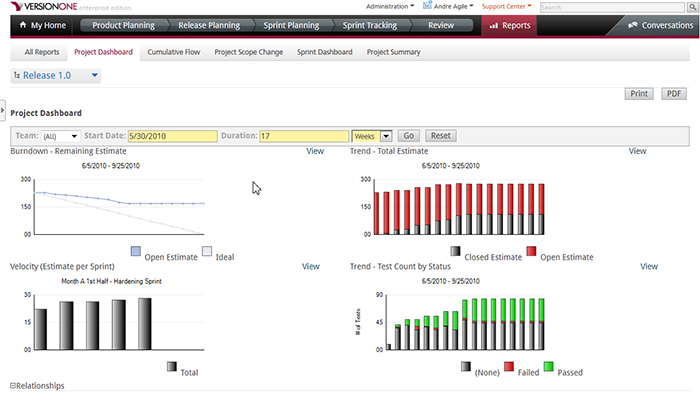
\includegraphics[scale=0.6]{ferramenta_versionone}
				\caption[Ferramenta VersionOne de Gestão de Requisitos]{Ferramenta VersionOne de Gestão de Requisitos.}
				\label{fig:ferramenta_versionone}
			\end{figure}

		\subsection[A Ferramenta Rally \emph{Software}]{A Ferramenta Rally \emph{Software}}
		\label{subsec:ferramenta_analise_rally}
			A ferramenta é fácil e agradável de utilizar. Ao realizar o cadastramento, informando o nome do projeto, bem como suas características, o grupo de Requisitos de \emph{Software} conseguiu obter facilmente uma visão das funcionalidades. A plataforma Rally reúne gerenciamento ágil de projetos, juntamente com os gerenciamentos de requisitos e defeitos. Dessa maneira, a equipe poderá contemplar uma imagem em tempo real dos compromissos do projeto.
			\\ \indent Como retratado anteriormente, o grupo da disciplina de Requisitos de \emph{Software} adotou a metodologia ágil para trabalhar com requisitos. De acordo com o processo que foi desenhado, é possível contemplar as funcionalidades requeridas na ferramenta.
			\begin{figure}[h]
				\centering
				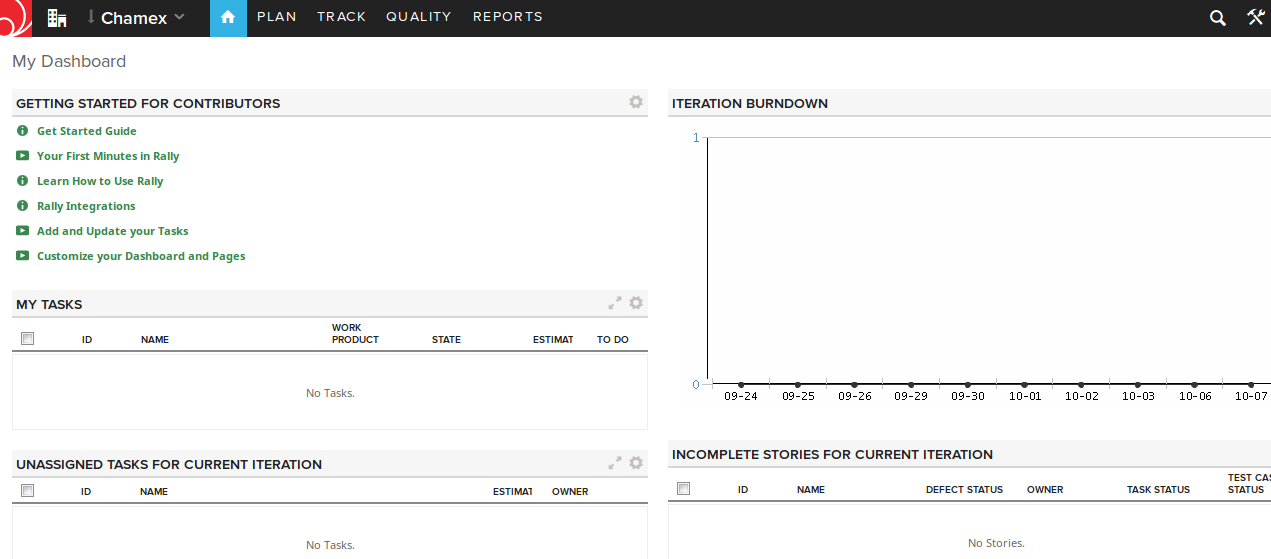
\includegraphics[scale=0.3]{ferramenta_rally}
				\caption[Ferramenta Rally \emph{Software} de Gestão de Requisitos]{Ferramenta Rally \emph{Software} de Gestão de Requisitos.}
				\label{fig:ferramenta_rally}
			\end{figure}

		\ \newline
		\subsection[Critérios Adotados para Avaliação]{Critérios Adotados para Avaliação}
		\label{subsec:ferramenta_analise_criterios}
			Para realizar uma escolha concisa de uma ferramenta para gerência de requisitos a ser utilizada neste trabalho, foi necessário estabelecer alguns critérios. Os critérios foram adotados segundo aspectos ergonômicos de \emph{software} \cite{ergolist} e, adicionalmente, aspectos de suporte das ferramentas às atividades da Engenharia de Requisitos. Inicialmente, a partir de indicações de monitores da disciplina de Requisitos de \emph{Software} e de leitura prévia de artigos, as ferramentas colocadas para investigação foram: VersionOne e Rally \emph{Software}. Os tópicos abaixo exibem os critérios adotados para avaliação das ferramentas:
			\begin{itemize}
				\item{\textbf{Multi-Plataforma}: Suporte da ferramenta em ser utilizada nos sistemas operacionais mais comuns (Windows, Linux e MacOS);}
				\item{\textbf{\emph{Web}}: Possibilidade do sistema em ser utilizado via \emph{web} através dos \emph{browsers} mais comuns (Internet Explorer, Mozilla Firefox, Opera e Google Chrome);}
				\item{\textbf{Cadastro de \emph{User Stories}}: Suporte do sistema para registro das \emph{user stories}, bem como alteração das informações de data, prioridade, resumo, critérios de aceitação, dentre outros;}
				\item{\textbf{Gerência de iterações}: Permissão para registrar iterações e associá-las às \emph{releases}, datas, pontuações de esforço, tempo gasto, dentre outros;}
				\item{\textbf{Visão do processo}: Capacidade da ferramenta em apresentar o fluxo de atividades;}
				\item{\textbf{Rastreabilidade}: Possibilidade da ferramenta em oferecer algum tipo de rastreabilidade, seja ela vertical ou horizontal;}
				\item{\textbf{Alocação de Recursos Humanos}: Permissão para alocar recursos humanos dentro das iterações de forma dinâmica;}
				\item{\textbf{Usabilidade}: Este critério avalia se a ferramenta é intuitiva, ou seja, de fácil utilização e não demanda alta quantidade de tempo para entender as suas funcionalidades e como utilizá-las;}
				\item{\textbf{Livre}: Ferramenta gratuita, sem ou com poucas limitações de recursos.}
			\end{itemize}

	\section[Escolha da Ferramenta de Gestão de Requisitos]{Escolha da Ferramenta de Gestão de Requisitos}
	\label{sec:ferramenta_escolha}
		As ferramentas apresentaram as mesmas funcionalidades, sendo que esse aspecto foi constatado em uma comparação. Contudo, a ferramenta Rally \emph{Software} apresenta uma versão, denominada \emph{Community}, que reúne os principais recursos avaliados e não há cobrança para utilização.
		\\ \indent A ferramenta VersionOne, embora possua vários recursos e uma boa usabilidade, após o período de 30 (trinta) dias, alguns recursos seriam retirados, prejudicando o desenvolvimento do trabalho.
		\\ \indent A Tabela \ref{table:comparativodeferramentas} descreve a comparação entre as duas ferramentas segundo os critérios adotados.

		\begin{table}[hp]
			\centering
			\begin{tabular}{|c|c|c|}
				\hline
				\textbf{Critérios} & \textbf{VersionOne} & \textbf{Rally \emph{Software}} \\ \hline
				Multi-Plataforma & \checkmark & \checkmark \\ \hline
				\emph{Web} & \checkmark & \checkmark \\ \hline
				Cadastro de \emph{User Stories} & \checkmark & \checkmark \\ \hline
				Gerência de Iterações & \checkmark & \checkmark \\ \hline
				Visão do Processo & \checkmark & \checkmark \\ \hline
				Rastreabilidade & \checkmark & \checkmark \\ \hline
				Alocação de Recursos Humanos & \checkmark & \checkmark \\ \hline
				Usabilidade & \checkmark & \checkmark \\ \hline
				Livre & X & \checkmark \\ \hline
			\end{tabular}
			\caption[Tabela de Comparação das Ferramentas]{Tabela de Comparação das Ferramentas.}
			\label{table:comparativodeferramentas}
		\end{table}